\documentclass[aps,pre,onecolumn,superscriptaddress,nofootinbib]{revtex4-2}
\usepackage{amsmath,amssymb,graphicx}
\renewcommand{\thefigure}{S\arabic{figure}}
\begin{document}
\title{Supplemental Material: Where forced defects go: fractional corner charges, images and screening in dimer coverings}
\author{Changyeon Won}
\affiliation{Department of Physics, Kyung Hee University, Seoul 02447, Republic of Korea}
\maketitle
Figures S1--S4 support Sec.~V of the main text (honeycomb lattice, armchair regions).
\begin{figure}[h]
\centering
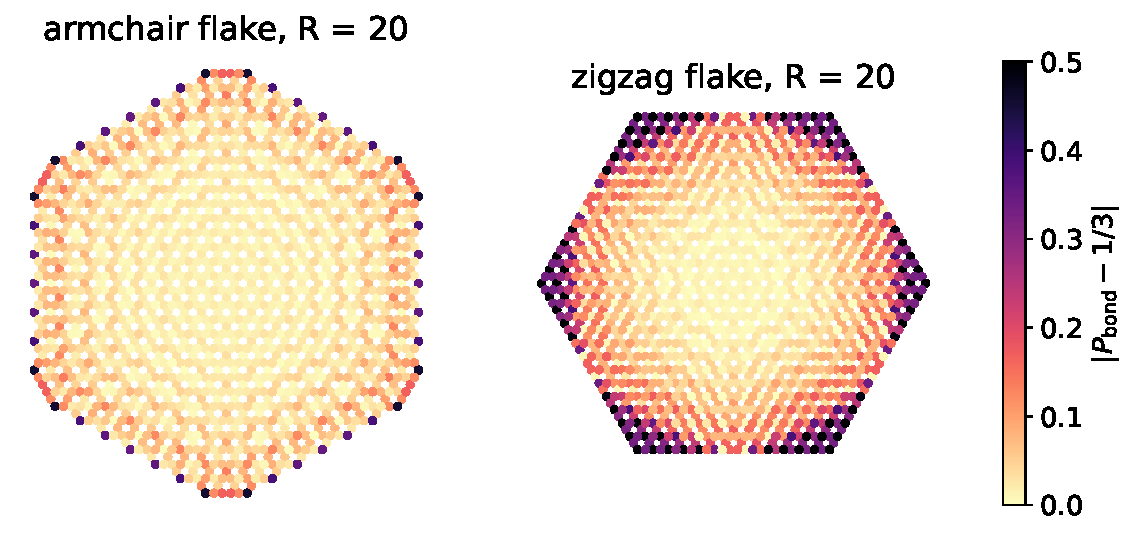
\includegraphics[width=0.6\textwidth]{figs/fig06_flatness.pdf}
\caption{Local deviation $|P-1/3|$ of the exact bond probabilities. Armchair flakes are flat liquids (core mean $0.035$, $0.017$, $0.012$ for $R=12,20,28$); zig-zag flakes (lozenge hexagons) freeze near the corners.}
\label{fig:flat}
\end{figure}

\begin{figure}[h]
\centering
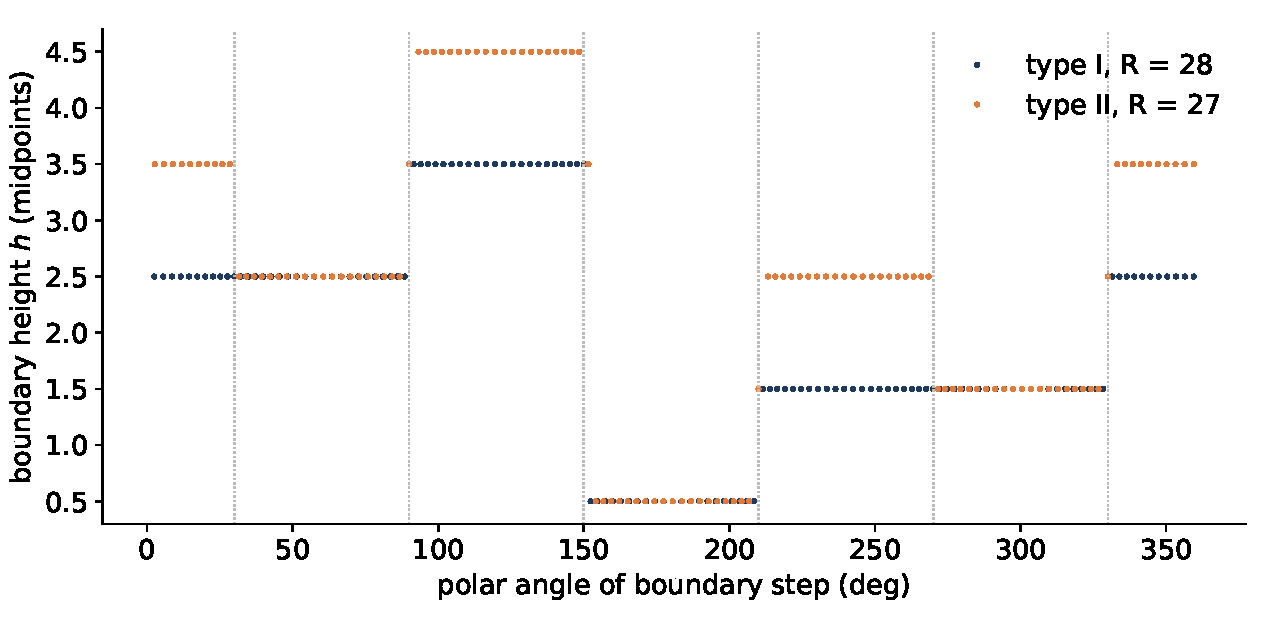
\includegraphics[width=0.6\textwidth]{figs/fig07_boundary_height.pdf}
\caption{Boundary height (step midpoints) around type I and type II hexagons with one forced defect. It is constant along each edge and jumps at the corners; the jump of $-3$ is the branch cut of the defect.}
\label{fig:height}
\end{figure}

\begin{figure}[h]
\centering
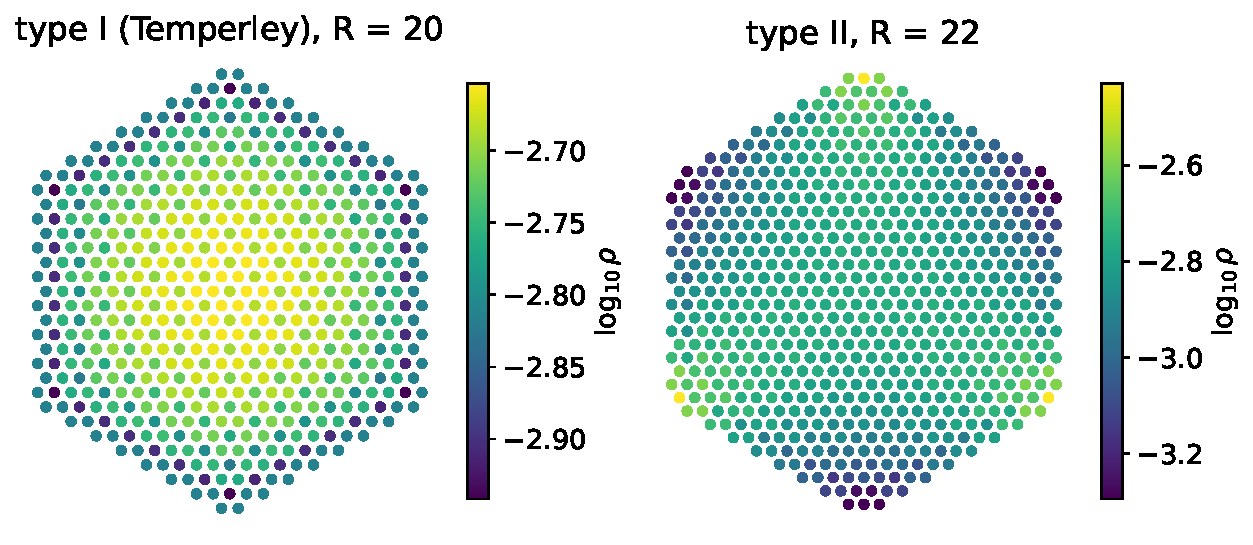
\includegraphics[width=0.6\textwidth]{figs/fig08_density.pdf}
\caption{Exact defect density on $A$ sites of a type I (left) and a type II (right) hexagon (separate colour scales). The type I density is uniform along the boundary and sixfold symmetric.}
\label{fig:density}
\end{figure}

\begin{figure*}[h]
\centering
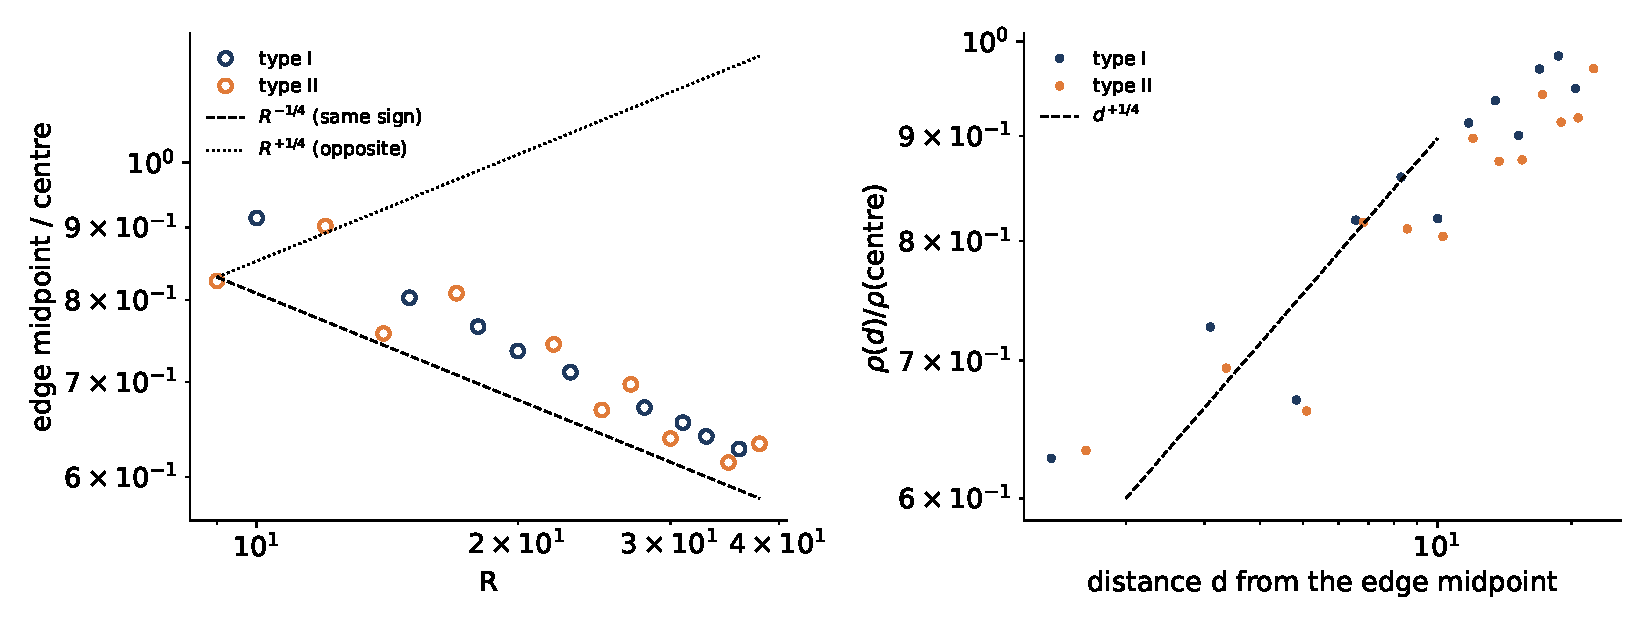
\includegraphics[width=0.85\textwidth]{figs/fig12_image.pdf}
\caption{Same-sign images on armchair edges. (a) Edge-midpoint to centre ratio against size; dashed: $R^{-1/4}$ (same sign), dotted: $R^{+1/4}$ (opposite sign). (b) Inward profile from the edge midpoint.}
\label{fig:image}
\end{figure*}

\end{document}
